\chapter{Introducción específica} % Main chapter title

\label{Chapter2}
%----------------------------------------------------------------------------------------
%	SECTION 1
%----------------------------------------------------------------------------------------
En este capítulo se hace una presentación de cuestiones técnicas particulares del trabajo, una descripción de alto nivel de las tecnologías involucradas en el desarrollo del trabajo, las herramientas que se utilizaron y servicios externos que formaron parte de la elaboración del trabajo, así también como los componentes de hardware empleados.

\section{Características de las soluciones existentes}

Es necesario, en primer lugar, hacer una introducción de las características que deben tener las soluciones de este tipo, junto con sus limitaciones y particularidades técnicas. Cualquier desarrollo de este tipo, debe considerarlas siguientes características para los módulos de hardware y software.

\subsection{Características del hardware}

Los botones antipánico y dispositivos geolocalizadores, suelen ser utilizados en zonas donde la cobertura de telefonía móvil es muy baja. Es decir, se cuenta con conectividad limitada para llamadas y mensajes, y prácticamente no hay cobertura para datos móviles, o es de baja tasa de transferencia. La tecnología más presente es la de GPRS o 2G\citep{NPERF:1}, ya que es la red de mayor alcance, pero también la de menor ancho de banda.
Esto impone una restricción respecto a la conectividad, por este motivo la mayoría de los dispositivos tienen las siguientes características respecto al método de comunicación:
\begin{itemize}
	\item Comunicación vía SMS, TCP o UDP para configuración y envío de datos.
	\item Comunicación vía protocolos personalizados\footnote{Existe una cantidad muy diversa de protocolos, desde protocolos binarios hasta protocolos en formato texto; puede consultarse el \href{https://www.traccar.org/protocols/}{listado de protocolos} que incorpora la plataforma \textit{open source} Traccar al respecto.} para reducir el \textit{overhead} de datos.
	\item Mecanismos para almacenar datos en caso de perder conectividad.
\end{itemize}

Debido a que dentro del alcance del trabajo se apunta a configuración y envío de mensajes de alerta, se consideró innecesario, para estas funciones, requerir otro medio adicional. No se considera apropiado usar un método de comunicación que pueda no ser fiable, como lo son los datos móviles en zonas donde la conectividad es baja.

Por otra parte, otro punto importante respecto a estos dispositivos, es su capacidad de obtener señal aceptable tanto de GSM como GNSS en ambientes \textit{indoor} y \textit{outdoor}. Prácticamente todos los botones antipánico poseen antenas internas y sin alimentación activa, por lo que su capacidad para adquirir un nivel de señal aceptable es limitada; esto introduce varios puntos a favor y en contra:
\begin{itemize}
	\item No generan un consumo de energía adicional.
	\item Su tiempo de \textit{startup}, es decir, hasta que adquieren un nivel de señal operativo aceptable, es elevado si están en ambientes cerrados.
	\item Su precisión suele ser baja en ambientes cerrados, lo cual puede ser un problema en situaciones de emergencia.
	\item El tiempo de actualización de la posición de la persona puede ser elevado si la antena no logra captar una buena señal.
\end{itemize}

\subsection{Características de los sistemas web}

Un sistema web, al requerir estar en comunicación con un dispositivo y mostrar su información en tiempo real, debe contar con las siguientes características, idealmente:
\begin{itemize}
	\item No requerir ningún software adicional para su acceso y uso más allá de un navegador web y conexión a Internet.
	\item Poder recibir mensajes de texto, es decir, tener un número telefónico virtual asociado.
	\item Enviar actualizaciones \textit{push} al navegador del usuario en tiempo real.
\end{itemize}

Se presentan algunos desafíos respecto al segundo y tercer punto. Para la recepción de SMS, es necesario tener integrada una central de telefonía virtual o implementar un \textit{Short Message Service Center} o SMSC, un servicio específico para el ruteo de mensajes de texto desde y hacia la web. Respecto al tercer punto, resulta obligatoria la implementación de algún mecanismo de actualización en tiempo real desde el servidor hacia el cliente, el navegador web, y no al revés, com puede ser \textit{WebSocket}.

En algunos casos, también debería permitir comunicación bidireccional con los dispositivos, para que un operador pueda configurarlos \textit{on-demand}. De todas maneras, debido a que está fuera del alcance del trabajo, no se planteó el desarrolo de esta característica.

\section{Componentes de hardware utilizados}

\subsection{Microcontrolador ESP32}

\begin{figure}[H]
	\centering
	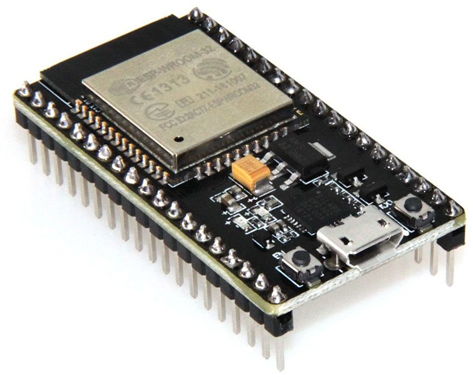
\includegraphics[width=.6\textwidth]{./Figures/esp32s.png}
	\caption{Microcontrolador ESP32-S}
	\label{fig:texmaker}
\end{figure}

Se utilizó un SoC (\textit{System on a Chip}) de la familia ESP32 de Espressif debido a que resulta una opción ideal para el desarrollo de sistemas embebidos y aplicaciones de Internet de las Cosas. Entre las características que resultaron más atractivas para su elección fueron\citep{ESP32:1}:
\begin{itemize}
	\item Bajo costo y disponibilidad en el mercado local.
	\item Prestaciones muy interesantes: Wi-Fi, Bluetooth, modos de ahorro de energía, varios periféricos, entre otros.
	\item Gran soporte de la comunidad y disponibilidad de bibliotecas, junto a su documentación.
	\item Ya utilizado en la carrera de especialización.
\end{itemize}

Se presenta a continuación algunas alternativas comparadas\footnote{La comparación debe ser interpretada linealmente ya que hay placas como Ai Thinker A9G y TTGO T-Call V1.3 que poseen ya módulos integrados, pero todos fueron analizados para el trabajo.}

\begin{table}[h]
	\centering
	\caption[Tabla comparativa]{Tabla comparativa de placas de desarrollo}
	\begin{tabular}{l c c c c}    
		\toprule
		\textbf{Característica} 	 & \textbf{ESP32} & \textbf{A9G} & \textbf{LoPy 4} & \textbf{TTGO T-Call}  \\
		\midrule
		Disponibilidad & Baja & No & No & Baja			\\		
		Comunidad & Muy grande & Grande & Poca & Si			\\
		Costo & Muy bajo & Moderado & Muy elevado & Muy elevado		\\
		Curva aprendizaje & Muy baja & Alta & Baja & Baja \\
		\bottomrule
		\hline
	\end{tabular}
	\label{tab:peces}
\end{table}


\subsection{Módulo GPS NEO-6M}

\begin{figure}[H]
	\centering
	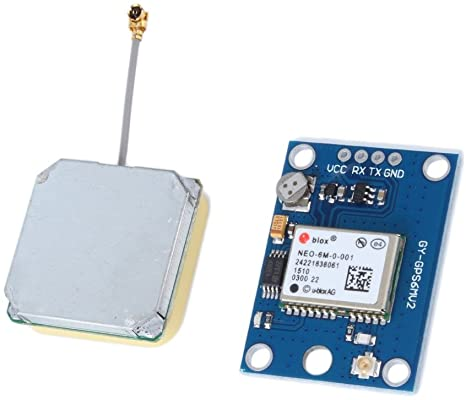
\includegraphics[width=.6\textwidth]{./Figures/neo-6m.jpg}
	\caption{Módulo GPS NEO-6M con una antena externa}
	\label{fig:texmaker}
\end{figure}

Para la implementación del módulo de posicionamiento, se decantó por el uso del módulo de GPS NEO-6M desarrollado por la compañía u-blox. Este módulo GPS posee un rango operativo de entre 2.7V y 3.6V, siendo muy similar al microcontrolador elegido anteriormente. Tiene modos de ahorro de energía configurables e interfaces de comunicación UART, SPI y I²C\citep{NEO6M:1}. Se analizaron otras alternativas, encontrando mucha similitudes, pero encontrando mayor documentación y casos de uso por parte de la comunidad para el NEO-6M.

Se muestra a continuación una tabla comparativa respecto a otro módulo similar:

\begin{table}[h]
	\centering
	\caption[Tabla comparativa]{Tabla comparativa de placas de desarrollo}
	\begin{tabular}{l c c}    
		\toprule
		\textbf{Característica} 	 & \textbf{Quectel L86} & \textbf{NEO-6M} \\
		\midrule
		Disponibilidad & Moderada & Baja			\\		
		Costo & Moderado & Elevado			\\
		Sistemas GNSS & GPS & GPS, GLONASS, Galileo		\\
		\bottomrule
		\hline
	\end{tabular}
	\label{tab:peces}
\end{table}

\subsection{Módulo GSM SIM800L}

\begin{figure}[H]
	\centering
	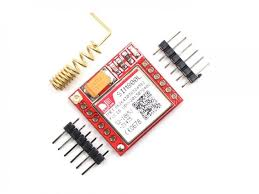
\includegraphics[width=.6\textwidth]{./Figures/sim800l.jpg}
	\caption{Módulo SIM800L}
	\label{fig:texmaker}
\end{figure}

Para el desarrollo de la conectividad a las redes de telefonía móvil, se utilizó el módulo SIM800L. SIM800L es un módulo de GSM desarrollado por la compañía Simcom. Funciona con un rango de voltaje entre 3.4V y 4.4V, y permite el uso del módulo mediante comandos AT\footnote{Un comando AT consiste en una cadena de caracteres corta utilizada dentro de la industria desde la década de 1980 hasta el día de hoy para la comunicación con módulos, módems, entre otros dispositivos{\citep{AT:1}.}}. Posee mecanismos para optimizar el consumo de energía pero tiene picos elevados de consumo durante la trasmisión. Respecto a la compatibilidad de generaciones de tecnologías de telefonía móvil, solo soporta hasta 2G\citep{SIM800L:1}. De todas maneras, para los fines del trabajo, resultó suficiente.

\subsection{Batería 18650 y chip cargador TP4056}

\begin{figure}[H]
\centering
\begin{minipage}{.5\textwidth}
  \centering
  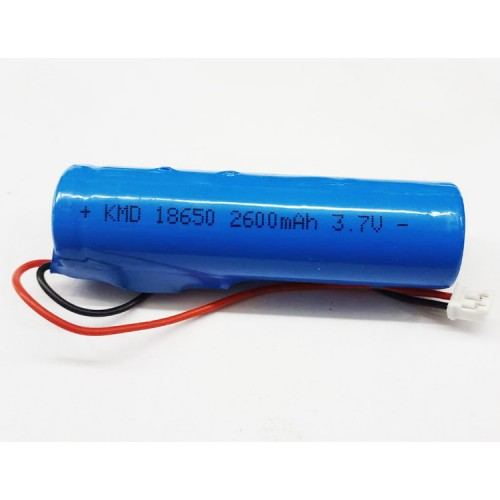
\includegraphics[width=.4\linewidth]{./Figures/18650.jpg}
  \captionof{figure}{Batería 18650}
  \label{fig:test1}
\end{minipage}%
\begin{minipage}{.5\textwidth}
  \centering
  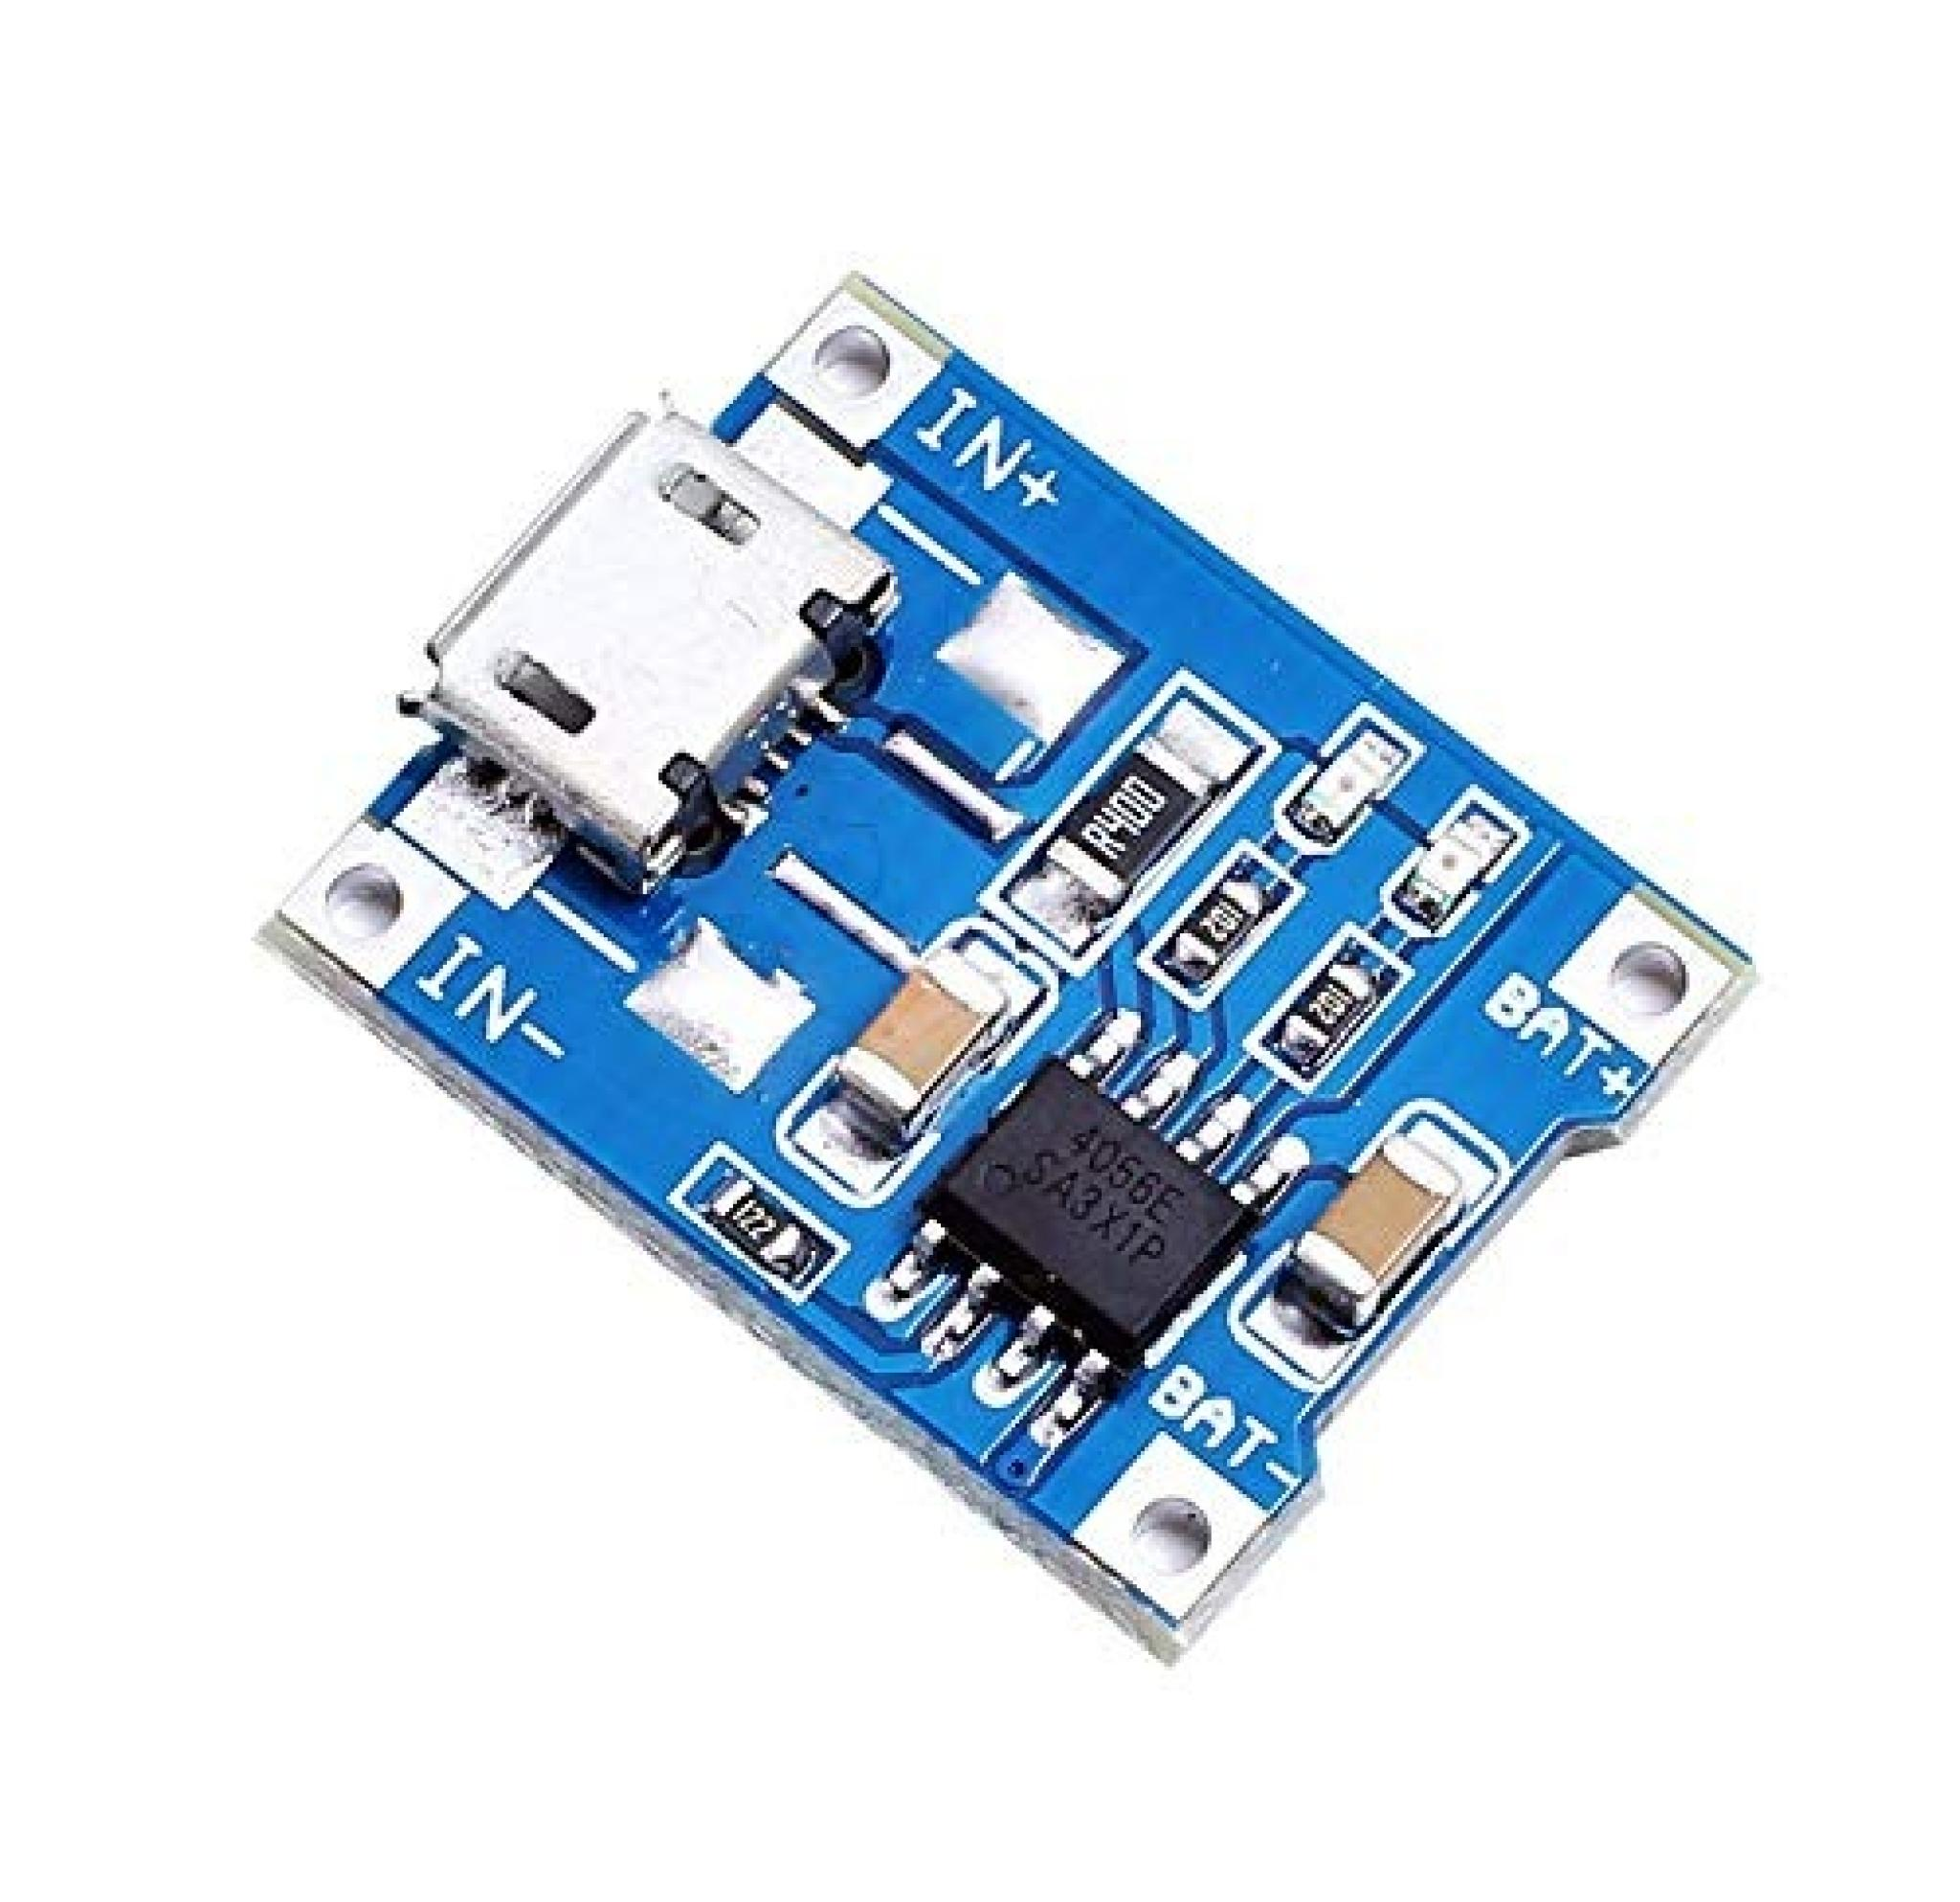
\includegraphics[width=.4\linewidth]{./Figures/tp4056.jpg}
  \captionof{figure}{Circuito Mp4056}
  \label{fig:test2}
\end{minipage}
\end{figure}

Para la alimentación del microcontrolador y sus módulos, se decidió utilizar una batería recargable del tipo 18650\footnote{El nombre 18650 es debido a las medidas de la batería: 18 indican su diámetro, 18 mm, mientras que el número 650 indica su longitud, que es 65 mm.} de Li-ion de 2600 mAh. Este tipo de baterías tiene la ventaja de trabajar con un rango de voltaje apropiado para microcontroladores y módulos, pudiendo además tener una elevada corriente máxiam de descarga (hasta 2 A aproximadamente).

Debido a que estas baterías requieren un circuito integrado para la carga y el control ante sobrecargas, se utilizó un módulo Tp4056 que permite la carga de la batería con una entrada micro USB de 5V, lo cual posibilita la carga con un cargador común de teléfono celular, por ejemplo.

\section{Componentes de software utilizados}

\subsection{Django REST framework}

Django REST framework es un conjunto de bibliotecas y herramientas del lenguaje Python para el desarrollo de aplicaciones web y APIs REST. Es el framework \textit{de facto} para el desarrollo web en Python. Entre sus características más interesantes, se encuentran\citep{DJANGO:1}
\begin{itemize}
	\item Soporte incluído para serialización de datos.
	\item Código modular y reusable mediante \textit{views} y \textit{viewsets}\footnote{En Django, las diferentes vistas o \textit{views} se agrupan en \textit{viewsets}} para definir interfaces REST sobre objetos.
	\item Mapeo de bases de datos relacionados a objetos mediante un \textit{Object–relational mapping} (ORM) propio.
	\item Documentación automática para las API por defecto.
	\item Estable desde hace más de una década.
	\item Combina la rapidez para el desarrollo y flexibilidad de un lenguaje de tipado dinámico junto a un conjunto de características y estructuras para escalar el desarrollo y que siga siendo mantenible.
	\item Soporte para múltiples mecanismos de autenticación ya incluídos.
	\item Bajo uso de recursos.
\end{itemize}

Se elegió Django para el desarrollo de la API de la aplicación porque se deseó trabajar con un lenguaje más dinámico, pero con un framework que posea ya una estructura para el desarrollo. Esto es debido a que la flexibilidad es un arma de doble filo para la evolución de los sistemas.

\begin{table}[h]
	\centering
	\caption[Tabla comparativa]{Tabla comparativa de frameworks web}
	\begin{tabular}{l c c}    
		\toprule
		\textbf{Característica} 	 & \textbf{Django} & \textbf{Express} \\
		\midrule
		Lenguaje & Python & Javascript \\		
		Curva de aprendizaje & Moderada & Muy baja			\\		
		Arquitectura & Definida & Flexible \\
		Enfoque & Estructurado & Libre/Flexible		\\
		Performance & Muy alta & Extremadamente alta \\
		Baterías incluídas\footnote{El término baterías incluídas se refiere a la disponibilidad por defecto de herramientas y bibliotecas útiles para el desarrollo.} & Sí & No \\
		\bottomrule
		\hline
	\end{tabular}
	\label{tab:peces}
\end{table}

\subsection{Angular}

Angular es un framework de código abierto desarrollado originalmente por Google para la construcción de aplicaciones web del tipo SPA\citep{ANGULAR:1}. Utiliza el lenguaje Typescript que es un superset de Javascript, dotándolo de tipado estático y características no presentes en Javascript. Entre sus características más potentes se pueden destacar\citep{ANGULAR:2}
\begin{itemize}
	\item Framework completo con una estructura definida.
	\item Arquitectura orientadas en componentes.
	\item \textit{Binding} de variables bidireccional.
	\item Disponibilidad de muchas bibliotecas y herramientas.
\end{itemize}

Para el desarrollo de las interfaces de usuario, se planteó el uso de \textit{Angular Material}, que es una biblioteca de componentes de interfaces disponible para Angular. Su principal ventaja es la disponibilidad de componentes estándar ya armados y diseño común\citep{ANGULAR:3}.

Para la incorporación de mapas en la aplicación, se definió el uso de Leaftlet, una biblioteca para el desarrollo de mapas en aplicaciones web. Su incorporación a Angular puede hacerse mediante el paquete \textit{ngx-leaftlet}\citep{LEAFLET:1} junto con el proveedor gratuito y \textit{open source} de mapas OpenStreetMap.

\subsection{PostgreSQL}

PostgreSQL es un \textit{relational database management system} o RDBMS de código abierto que hace uso de SQL y es famoso por ser \textit{ACID-compliant}, su gran amplitud de tipos de datos, robustez y extensibilidad\citep{POSTGRES:1}. Es uilizado ampliamente por la industria del software\citep{POSTGRES:2} y se encuentra disponible como una opción por los mayores proveedores de \textit{cloud} de la actualidad. Prácticamente todos los frameworks web permiten conectarse a este motor de bases de datos. 

\subsection{Heroku}

Heroku es un proveedor de infraestructura y servicios en la nube y \textit{Platform as a Service} (PaaS) focalizado en el rápido despliegue y mantenimiento de las aplicaciones web. La principal ventaja de Heroku es que apunta a abstraer al usuario de detalles técnicas y la infraestructura que da soporte a los serivcios usados.

Se presenta una breve tabla comparativa frente a otros proveedores, como Amazon Web Services (AWS) y Google Cloud Platform (GCP).
\begin{table}[h]
	\centering
	\caption[Tabla comparativa]{Tabla comparativa de proveedores \textit{cloud}}
	\begin{tabular}{l c c c}    
		\toprule
		\textbf{Característica} 	 & \textbf{Heroku} & \textbf{AWS} & \textbf{GCP} \\
		\midrule
		Complejidad & Baja & Muy alta & Media-Alta \\		
		Costo & Medio & Bajo & Bajo-Medio			\\		
		Flexibilidad & Baja-Media & Muy alta & Alta \\
		Servicios & Poca oferta & Mucha oferta & Mucha oferta 	\\
		Regiones & Limitadas & Amplias & Amplias \\
		\bottomrule
		\hline
	\end{tabular}
	\label{tab:peces}
\end{table}

\section{Herramientas y servicios de software utilizados}

\subsection{Docker}

Docker es una plataforma \textit{open source} para la contenerización de aplicaciones, con el objetivo de\citep{DOCKER:1}:
\begin{itemize}
	\item Generar versiones de sistemas idénticas entre diferentes ambientes, es decir que un sistema sea portable.
	\item Aislar los recursos del \textit{host} de los sistemas que corren en él.
	\item Reducir los tiempos de despliegue, mantenimiento y soporte de aplicaciones.
\end{itemize}

Docker permite generar imágenes de sistemas siguiendo un conjunto de instrucciones definidos mediante un archivo \textit{Dockerfile}, habilitando generar estas mismas imágenes en otros ambientes.

\subsection{Visual Studio Code}

\textit{Visual Studio Code} es un editor de texto e IDE (Integrated development environment o Entorno de desarrollo integrado) de código abierto desarrollado originalmente por Microsoft\citep{VSCODE:1}. Su flexibilidad y soporte para una cantidad considerable de extensiones para gran parte de los lenguajes y frameworks de la industria lo posicionó en la última década como uno de los IDE más utilizados.

Permite desarrollar aplicaciones con Python, Javascript/Typescript, incorporando incluso frameworks para sistemas embebidos como ESP-IDF o Platform.IO desarrollo embebidos como es el framework ESP-IDF o PlatformIO\footnote{Ver \href{https://platformio.org/install/ide?install=vscode}{Installation · PlatformIO} o \href{https://docs.espressif.com/projects/esp-idf/en/v4.2.3/esp32/get-started/vscode-setup.html}{Getting started with ESP-IDF VS Code - ESP32}.}. La mayoría de proveedores de servicios en la nube han desarrollado extensiones para agilizar el despliegue de aplicaciones en sus servicios.

\subsection{PyGPSClient}

\begin{figure}[H]
	\centering
	\includegraphics[width=.9\textwidth]{./Figures/pygpsclient.png}
	\caption{Aplicación PyGPSClient}
	\label{fig:texmaker}
\end{figure}

PyGPSClient es una herramienta de escritorio disponible desarrollada en Python para el \textit{debugging} y análisis de varios módulos GNSS de u-blox. Su principal ventaja frente a la herramienta estándar para las pruebas de estos módulos, u-center, es que está disponible para cualquier sistema que soporte Python, en comparación de la anterior que solo está disponible para Windows\citep{PYGPSCLIENT:1}.

\subsection{Moserial}

\begin{figure}[H]
	\centering
	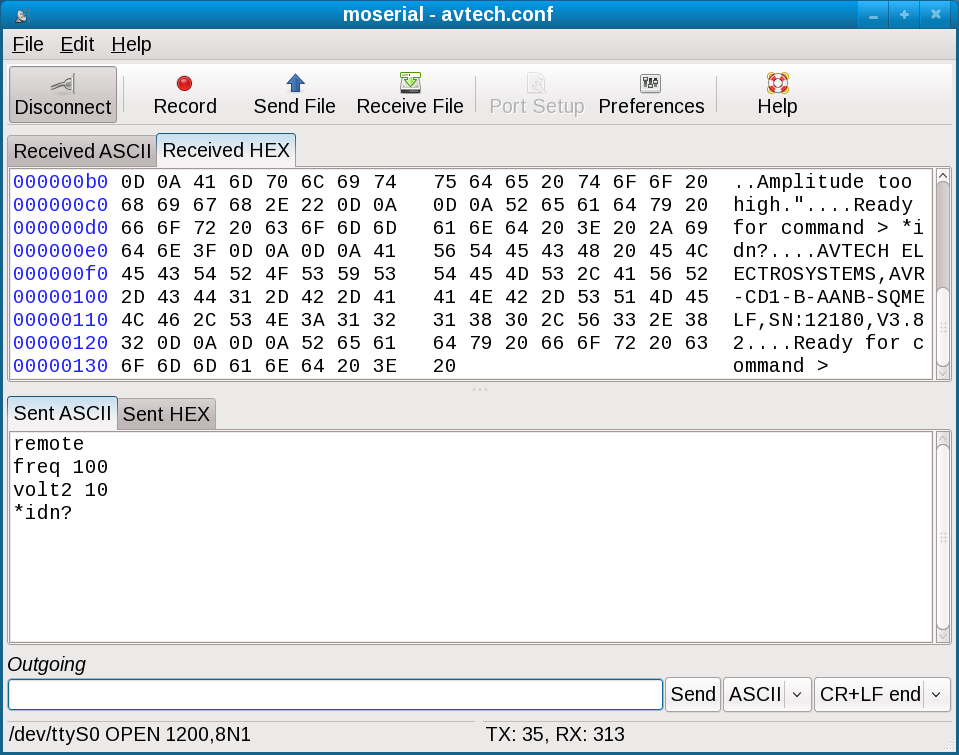
\includegraphics[width=.9\textwidth]{./Figures/moserial.png}
	\caption{Aplicación Moserial}
	\label{fig:texmaker}
\end{figure}

Moserial es una aplicación de escritorio orientada al \textit{testing} de dispositivos embebidos, consolas y equipos electrónicos que permiten comunicación vía \textit{Universal Asynchronous Receiver-Transmitter} o UART. Se encuentra disponible para el entorno gráfico GNOME, popular en sistemas GNU/Linux. Su uso resultó de importancia para la comunicación con el módulo de GSM, SIM800L.

\subsection{Twilio}

Twilio es un \textit{Communications Platform as a Service} o CPaSS que ofrece diferentes servicios y herramientas para el desarrollo de sistemas que requieran funcionalidades relacionadas a telefonía IP, envío y recepción de mensajes de texto, accediendo a dicho servicios mediante varios mecanismos ofrecidos por la plataforma, como APIs web\citep{TWILIO:1}. Dentro del trabajo, su principal uso fue para la adquisición de un número de teléfono virtual para la recepción de mensajes de texto provinientes de un dispositivo embebido.
